\documentclass[dvipsnames,tikz]{standalone}
\usepackage{amsmath}
\usepackage{arevmath}
\usepackage{xcolor}
\usepackage{tikz}
\usetikzlibrary{calc}
\usetikzlibrary{decorations.pathreplacing,calligraphy,3d}
\usetikzlibrary{lindenmayersystems}

\tikzset{main/.style={draw=black, circle, color=black}}


\begin{document}
	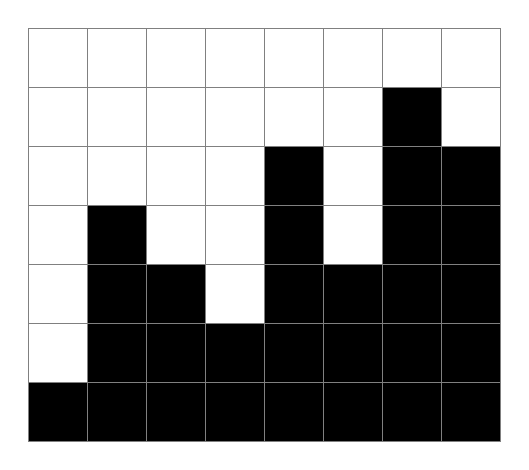
\begin{tikzpicture}[scale=0.75, main, line join=bevel]
		\fill (0,0) -- (8,0) -- (8,5) -- (7,5) -- (7,6) -- (6,6) -- (6,3) -- (5,3) --(5,5) --(4,5) -- (4,2) -- (3,2) -- (3,3) -- (2,3) -- (2,4) -- (1,4) -- (1,1) -- (0,1) -- cycle;
		\draw[main, gray] (0,0) grid (8,7);
	\end{tikzpicture}
	
	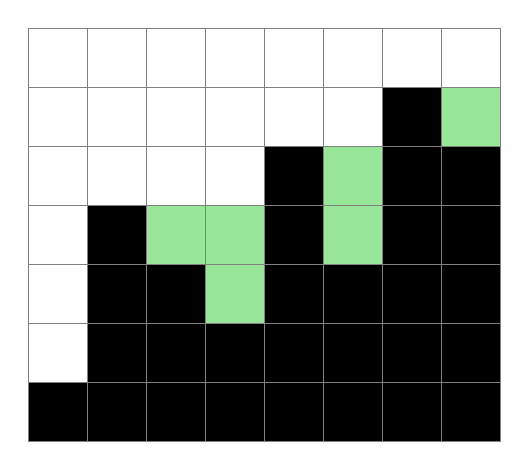
\begin{tikzpicture}[scale=0.75, main, line join=bevel]
		\fill (0,0) -- (8,0) -- (8,5) -- (7,5) -- (7,6) -- (6,6) -- (6,3) -- (5,3) --(5,5) --(4,5) -- (4,2) -- (3,2) -- (3,3) -- (2,3) -- (2,4) -- (1,4) -- (1,1) -- (0,1) -- cycle;
		\fill[LimeGreen, semitransparent] (8,5) -- (8,6) -- (7,6) -- (7,5) -- cycle;
		\fill[LimeGreen, semitransparent] (6,3) -- (6,5) -- (5,5) -- (5,3) -- cycle;
		\fill[LimeGreen, semitransparent] (4,2) -- (4,4) -- (2,4) -- (2,3) --(3,3) -- (3,2) -- cycle;
		\draw[main, gray] (0,0) grid (8,7);
	\end{tikzpicture}
\end{document}